%Dies ist die Hauptseite des Dokumentes. Es werden u. a. alle Kapitel,
%Einstellung im Header eingebunden.  Veränderungen müssen in folgenden Dateien
%vorgenommen werden:
      %- Layout.tex
      %- newComments.tex
      %- Titelseite
      %- Versionsübersicht
      %- einzelne Kapitel (evtl. erweitern)


% Definition von globalen Parametern, die derzeit auf der Titelseite und in der
% Kopfzeile verwendet werden. Der in <> gesetzte Text ist zu verändern.

\newcommand{\praktikumTitel}{WiReLib}
\newcommand{\projektTitel}{WiReLib}


%Hier sind alle Einstellungen enthalten, die sich auf das Seiten- und
%Dokumentenlayout beziehen

\documentclass[
  11pt,                % Schriftgröße
  DIV12,
  german,              % für Umlaute, Silbentrennung etc.
  oneside,            % einseitiges Dokument
  titlepage,          % es wird eine Titelseite verwendet
  parskip=half,        % Abstand zwischen Absätzen (halbe Zeile)
  headings=normal,      % Größe der Überschriften verkleinern
  captions=tableheading,  % Beschriftung von Tabellen unterhalb ausgeben
  final                % Status des Dokuments (final/draft)
]{scrreprt}            %


%------Ändern von Schriftschnitten - (Muss ganz am Anfang stehen !) ------------
\usepackage{fix-cm}

%------Umlaute -----------------------------------------------------------------
%   Umlaute/Sonderzeichen wie äüöß können direkt im Quelltext verwenden werden.
%    Erlaubt automatische Trennung von Worten mit Umlauten.
\usepackage[T1]{fontenc}
\usepackage[utf8]{inputenc}

%------Anpassung der Landessprache----------------------------------------------
\usepackage{ngerman}

%------Einfache Definition der Zeilenabstände und Seitenränder------------------
\usepackage{geometry}
\usepackage{setspace}
\usepackage{xspace}

%------Schriftgrößenanpassung von einzelnen Textpassagen------------------------
\usepackage{relsize}

%------Trennlinien in Kopf- und Fusszeile
\usepackage[headsepline, footsepline, ilines]{scrpage2}

%------Grafiken-----------------------------------------------------------------
\usepackage{graphicx}

%------Packet zum Sperren, Unterstreichen und Hervorheben von Texten------------
\usepackage{soul}

%------ergänzende Schriftart----------------------------------------------------
\usepackage{helvet}

%------Lange Tabellen-----------------------------------------------------------
\usepackage{longtable}
\usepackage{array}
\usepackage{ragged2e}
\usepackage{lscape}

%------PDF-Optionen-------------------------------------------------------------
\usepackage[
  bookmarks,
  bookmarksopen=true,
  colorlinks=true,
  linkcolor=black,        % einfache interne Verknüpfungen
  anchorcolor=black,      % Ankertext
  citecolor=black,        % Verweise auf Literaturverzeichniseinträge im Text
  filecolor=black,        % Verknüpfungen, die lokale Dateien öffnen
  menucolor=black,        % Acrobat-Menüpunkte
  urlcolor=black,         % Farbe für URL-Links
  backref,                % Zurücktext nach jedem Bibliografie-Eintrag als
                          % Liste von Überschriftsnummern
  pagebackref,            % Zurücktext nach jedem Bibliografie-Eintrag als
                          % Liste von Seitenzahlen
  plainpages=false,       % zur korrekten Erstellung der Bookmarks
  pdfpagelabels,          % zur korrekten Erstellung der Bookmarks
  hypertexnames=false,    % zur korrekten Erstellung der Bookmarks
  linktocpage             % Seitenzahlen anstatt Text im Inhaltsverzeichnis
                          % verlinken
  ]{hyperref}

%-----Glossar-Optionen----------------------------------------------------------
\usepackage{translator}
\usepackage[				   %
acronym,		% ein Abkürzungsverzeichnis erzeugen
toc,			% Taucht im Inhaltsverzeichnis auf
]				   
{glossaries}
\makeglossaries

\usepackage{xcolor}
\definecolor{lightergray}{rgb}{0.9,0.9,0.9}

\usepackage{listings}
\lstset{numbers=left, numberstyle=\tiny, numbersep=5pt,
breaklines=true, backgroundcolor=\color{lightergray},
basicstyle=\ttfamily,
}
\usepackage{booktabs}
      % enthält eingebundene Packete

%------Seitenränder-------------------------------------------------------------
\geometry{verbose,                     % zeigt die eingestellten Parameter beim
                                       % Latexlauf an
      paper=a4paper,                   % Papierformat
      top=25mm,                        % Rand oben
      left=25mm,                       % Rand links
      right=25mm,                      % Rand rechts
      bottom=45mm,                     % Rand unten
      pdftex                           % schreibt das Papierformat in die
                                       % Ausgabe damit Ausgabeprogramm
                                       % Papiergröße erkennt
  }

%Seitenlayout
\onehalfspace        % 1,5-facher Abstand

%------Kopf- und Fußzeilen -----------------------------------------------------
\pagestyle{scrheadings}

%------Kopf- und Fußzeile auch auf Kapitelanfangsseiten ------------------------
\renewcommand*{\chapterpagestyle}{scrheadings}

%------Schriftform der Kopfzeile -----------------------------------------------
\renewcommand{\headfont}{\normalfont}

%------Kopfzeile----------------------------------------------------------------
\setlength{\headheight}{21mm}        % Höhe der Kopfzeile
\ihead{\large{\textsc{\praktikumTitel}}\\    % Text in der linken Box
       \small{\projektTitel}}
\chead{}                            % Text in der mittleren Box

%----Fusszeile
\cfoot{}                            % Text in mittlerer Box
\ofoot{\pagemark}                    % Seitenzahl in rechter Box
          % Diese Datei enthält alle
                                          % Layouteinstellungen

% Dieses Befehle sortieren die Einträge in den einzelnen Listen:
%makeindex -s datei.ist -t datei.alg -o datei.acr datei.acn
%makeindex -s datei.ist -t datei.glg -o datei.gls datei.glo
%makeindex -s datei.ist -t datei.slg -o datei.syi datei.syg

% Kapitel 9
%-------------------------------------------------------------------------------
%Hier werden Fachbegriffe und Abkürzungen erklährt.
% Verwendet werden diese Begriffe mit \gls{name} oder \Gls{name} wenn der Anfang
% groß geschrieben sein muss.
%
%%	Beispiel unter: http://ewus.de/tipp-1029.html
%%	und natürlich Erkärung mit dem Befehl
%texdoc glossaries

\newacronym{UB}{UB}{Universitätsbibliothek}
\newacronym{GITZ}{GITZ}{Gauß-IT-Zentrum}
\newacronym{LDAP}{LDAP}{Lightweight Directory Access Protocol\protect\glsadd{glos:LDAP}}

% nur über \gls{LDAP} verwenden.
\newglossaryentry{glos:LDAP}{name=Lightweight Directory Access Protocol,
description={LDAP ist ein Verzeichnisdienst der von der TU Braunschweig für die Benutzerauthentifizierung bereit gestellt wird}
}
\newglossaryentry{glos:https}{name=Hypertext Transfer Protocol Secure,
description={Hypertext Transfer Protocol Secure ist die verschlüsselte Variante
vom Hypertext Transfer Protocol und ist eine zertifiktasbasierende sichere
Übertragungstechnik}
}
\newglossaryentry{glos:sqlite}{name=SQLite,
description={SQLite ist eine Relationale Datenbank die von Python direkt zur Verfügung gestellt wird}
}
\newglossaryentry{glos:copdes}{name=Corporate Design,
description={Das Corporate Design ist das gemeinsame Erscheinungsbild eine Unternehmens. Dies bezieht sich unter anderem auf Kommmunikationsmittel, Werbemittel und Internetauftritte}
}
\newglossaryentry{glos:unicode}{name=Unicode,
description={Der Unicode ist ein Standard, in dem jedes sinntragende Schirftzeichen einem digitalen Code zugeordnet werden soll. Dadurch sollen Kompatibilitätsproblem aufgrund verschiedener Kodierungen in verschiedenen Ländern umgangen werden}
}
\newglossaryentry{glos:thmefi}{name=Thunderbird Message Filter,
description={Der Thunderbird Message Filter ist eine einfache Möglichkeit E-Mails in dem Programm Mozilla Thunderbird zu durchsuchen}
}
\newglossaryentry{glos:BibTeX}{name=Bib\TeX,
description={Bib\TeX\xspace ist ursprünglich eine Erweiterung für \LaTeX\xspace zur Verwaltung eines Literaturverzeichnisses für wissenschaftliche Publikationen. Inzwischen ist das Format auch unter anderen Textverarbeitungsprogrammen benutzbar}
}
\newglossaryentry{glos:Allegro}{name=Allegro,
description={Allegro ist das Datenbanksystem, welches in der Universitätsbibliothek der TU Braunschweig entwickelt und verwendet wird}
}
\newglossaryentry{glos:regex}{name=Reguläre Ausdrücke,
description={Reguläre Ausdrücke sind ein Mittel der Theoretischen Informatik um Sprachen (dt. Wortmengen) zu beschreiben. In der angewanten Informatik werden diese Ausdrücke noch heute oft verwendet. Mit Regulären Ausdrücken ist eine präzise Beschreibung eines Suchwortes möglich}
}
\newglossaryentry{glos:ext}{name=Externe,
description={Der Begriff \emph{Externe} beschreibt alle Personen die nicht am System angemeldet sind, also \mbox{z.\,B.}\xspace Mitarbeiter anderer Institute mit einem Ausleihwunsch}
}



\newcommand{\BibTeX}{\gls{glos:BibTeX}\xspace}
%------Beginn des Gesamtdokumentes----------------------------------------------
\begin{document}

%------Eingebundene Seiten, Verzeichnisse bzw. Kapitel--------------------------
% Dies ist die Titelseite des Grobentwurfs.
% Die in "<...>" sind zu ersetzen
% Die Ausgabe darf 1 Seite nicht überschreiten, also ggf. Abstände anpassen
% Die Angabe in [...] gibt den Abstand nach der entsprechenden Zeile an.


%----Stil dieser Seite----------------------------------------------------------
\thispagestyle{plain}      % Kopfzeile bleibt leer

%----Beginn der Titelseite------------------------------------------------------
\begin{titlepage}

%----zentrierte Ausrichtung über die gesamte Seite----------------------------
\begin{center}

%----Titel des Praktikum (\praktikumTitel in newComments zu verändern)--------
{\relsize{4}{\textbf{\textsc{\praktikumTitel}}}}\\[3ex]%[5ex]

%----Titel des Teilprojektes (\projektTitel in newComments verändern)---------
{\relsize{3}{\textbf{\textsc{\projektTitel}}}}\\[3ex]%[5ex]

Software-Entwicklungspraktikum (SEP)\\
Sommersemester 2012\\[4ex]%[6ex]

{\relsize{3}\so{\textbf{Grobentwurf}}}\\[4ex]%[5ex]

%----eingebundenes Logo der TU--------------------------------------------------

\includegraphics[scale=0.8]{bilder/carolo.jpg}\\[4ex]%[5ex]

%----Daten des Auftraggebers
Auftraggeber\\
Technische Universität Braunschweig\\
Wissenschaftliches Rechnen\\
Prof. Hermann G. Matthies\\
Hans-Sommer-Straße 65\\
D-38092 Braunschweig\\[1ex]%[2ex]
Betreuer: Elmar Zander\\[4ex]%[5ex]

% ----Tabelle der Praktikumsteilnehmer------------------------------------------
Auftragnehmer:
\begin{tabular}{l<{\hspace{20mm}} l<{\hspace{30mm}}}\\
  Name                   &   E-Mail-Adresse\\      % Zeilenüberschift
  \hline                    % Linie unterhalb der Zeilenüberschrift
  %----Nachfolgend alle Namen und E-Mail-Adressen der Teilnehmer einfügen
  Eric Anders 		& eric.anders89@web.de\\
  Johann Hong 		& johann.hong@googlemail.com\\
  Jörn Hameyer 		& j.hameyer@tu-bs.de\\
  Marco Melzer 		& marco.melzer@tu-braunschweig.de\\
  Markus Dietrich 	& markus.dietrich@tu-bs.de\\
  Philipp Offensand & PhilippOffensand@gmx.de\\
  Stephan Sobol 	& stephan.sobol@web.de\\
  Theodor van Nahl 	& t.nahl@tu-bs.de
\end{tabular}\\[1ex]%[2ex]

Braunschweig, 24.04.2012

\end{center}
\end{titlepage}

                      % Titelseite
%Diese Datei dient der Versionskontrolle. Sie ist vollständig zu bearbeiten.

%----Überschrift------------------------------------------------------------
{\relsize{2}\textbf{Versionsübersicht}}\\[2ex]

%----Start der Tabelle------------------------------------------------------
\begin{longtable}{|m{1.78cm}|m{1.59cm}|m{2.86cm}|m{1.9cm}|m{5.25cm}|}

  \hline                                              % Linie oberhalb

  %----Spaltenüberschriften------------------------------------------------
  \textbf{Version}  &    \textbf{Datum}  &    \textbf{Autor}  &
  \textbf{Status}   &    \textbf{Kommentar}       \\  %Spaltenüberschrift
  \hline                                              % Gitterlinie

  %----die nachfolgeden beiden Zeilen so oft wiederholen und die ... mit den
  %    entsprechenden Daten zu füllen wie erforderlich
  0.1   &    16.05.2012    &    Theodor van-Nahl    &   in Bearbeitung     &    Analyse der Produktfunktionen F100-F200\\       % Eintrag in Zeile
  \hline                                              % Gitterlinie unten
  0.2   &    17.05.2012    &    Jörn Hameyer    &   in Bearbeitung     &    Analyse der Produktfunktionen F226-F229\\       % Eintrag in Zeile
  \hline
  0.3   &    18.05.2012    &    Stephan Sobol    &   in Bearbeitung     &    Analyse der Produktfunktionen F220-F225\\       % Eintrag in Zeile
  \hline
  0.4   &    18.05.2012    &    Philipp \mbox{Offensand}    &   in Bearbeitung     &    Qualitätsanalyse\\       % Eintrag in Zeile
  \hline
  0.5   &    18.05.2012    &    Markus Dietrich    &   in Bearbeitung     &    Analyse der Produktfunktionen F230-F302\\       % Eintrag in Zeile
  \hline
  0.6   &    18.05.2012    &    Johann Hong    &   in Bearbeitung     &    Analyse der Produktfunktionen F210-F214\\       % Eintrag in Zeile
  \hline
  0.7   &    18.05.2012    &    Marco Melzer    &   in Bearbeitung     &    Einleitung\\       % Eintrag in Zeile
  \hline
  0.8   &    18.05.2012    &    Philipp \mbox{Offensand}    &   in Bearbeitung     &    Komponentenspezifikation\\       % Eintrag in Zeile
  \hline
  0.9   &    19.05.2012    &    Theodor van-Nahl    &   in Bearbeitung     &    Analyse der Produktfunktion F201-F210\\       % Eintrag in Zeile
  \hline
  0.10   &   21.05.2012    &    Marco Melzer    &   in Bearbeitung     &    Schnittstellenspezifikation\\       % Eintrag in Zeile
  \hline
  0.11   &   22.05.2012    &    Joahann Hong    &   in Bearbeitung     &    Verteilungsentwurf\\       % Eintrag in Zeile
  \hline
  0.12   &   23.05.2012    &    Jörn Hameyer,\newline Stephan Sobol    &   in Bearbeitung     &    Protokolle für die Benutzung der Komponenten\\       % Eintrag in Zeile
  \hline
  1.0   &    23.05.2012    &    sämtliche Auftragnehmer    &   abgenommen     &    \\       % Eintrag in Zeile
  \hline
  

%----Ende der Tabelle------------------------------------------------------
\end{longtable}

Status: "`in Bearbeitung"' oder "`abgenommen"'
Kommentar: hier eintragen, was ge\"andert bzw. ergänzt wurde


Hinweis zum Template:
Dieses Template enth\"ult Hinweise, die alle kursiv geschrieben sind. Alles
Kursivgeschriebene ist selbstverst\"andlich bei Abgabe zu entfernen sind.
Angaben in <\ldots> sind mit dem entsprechendem Text zu f\"ullen.  \"Uberz\"ahlige
Kapitel, d.h. Kapitel, die nicht bearbeitet werden m\"ussen, da sie nicht der
Aufgabenstellung entsprechen, bitte entfernen.

Aufgabe des Grobentwurfs: Aufgabe dieses Dokumentes ist es, die Architektur des
Systems zu beschreiben und die daraus resultierenden Pakete durch die
Definition von Schnittstellen zu Komponenten auszubauen.
       % Versionsübersicht

\tableofcontents                          % Inhaltsverzeichnis wird automatisch
                                          % generiert
\listoffigures                            % ebenso das Abbildungsverzeichnis

Abbildung 1: Aktivitätsdiagramm Projektdetails  5 \\
Abbildung 2: Verteilung von <ID>  7       \\
Abbildung 3: Sequenzdiagramm für <ID>  7  \\
Abbildung 4: Komponentendiagramm  8       \\
Abbildung 5: Protokollstatechart für jede Komponente  9    \\
Abbildung 6: Verteilungsdiagramm  10      \\




%----Kapitel des Feinentwurfs, die mit Inhalt zu füllen sind--------------------
% Kapitel 1
% Die Unterkapitel können auch in separaten Dateien stehen,
% die dann mit dem \include-Befehl eingebunden werden.
%-------------------------------------------------------------------------------

\chapter{Einleitung}
Die Datenbank WiReLib repräsentiert die den Bestand der Bibliothek für das Institut für Wissenschaftliches Rechnen.
Auf diese Datenbank können Nutzer über ein Web-Interface zugreifen um Dokumente zu suchen und sich nach der Anmeldung Dokumente auszuleihen.

\section{Projektdetails}
Die Funktionalitäten gliedern sich in drei Teilbereiche.
Diese Bereiche bündeln die Anforderungen, die im Pflichtenheft spezialisiert
worden sind.

\begin{figure}[h]
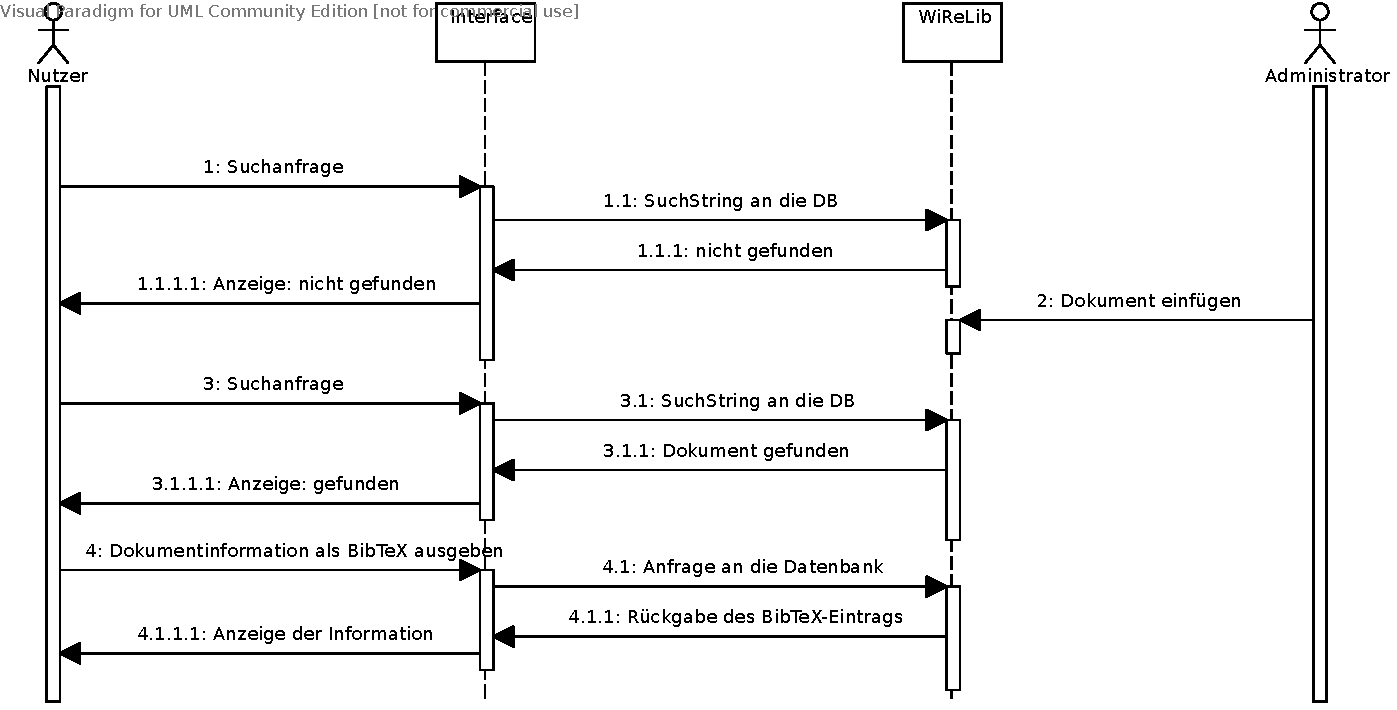
\includegraphics[width=0.8\linewidth]{bilder/Seq-Uebersicht.pdf}
\caption[Übersichtssequenzdiagramm]{Übersichtssequenzdiagramm}
\label{fig:Seqü}
\end{figure}

\subsection{Client}
Über das Web-Interface erhält der als Client fungierende Browser Zugriff auf die Datenbank und kann verschiedene Funktionen nutzen.

\subsection{Server}
Auf dem Server läuft die Anwendung, welche verschiedene Funktionen zum Auslesen und Verwalten der Datenbank bereitstellt. 
Auch stellt der Server die Datenbank bereit und baut eine sichere Verbindung zum Client auf.

\subsection{Datenbank}
In der Datenbank werden die Dokumenente sowie die Nutzerrechte verwaltet.
Auch werden Daten zu den einzelnen Nutzern gespeichert um diese zu identifizieren und im Falle des Ablaufs der Verleihfrist zu benachrichtigen.
                % Kapitel 1
% Kapitel 2 mit den entsprechenden Unterkapiteln
% Die Unterkapitel können auch in separaten Dateien stehen,
% die dann mit dem \include-Befehl eingebunden werden.
%-------------------------------------------------------------------------------
\chapter{Analyse der Produktfunktionen}

Dieser Abschnitt stellt die Basis für die Festlegung der Architektur dar. Die
Festlegung einer geeigneten Architektur geschieht aufgrund der im Pflichtenheft
analysierten Produktfunktionen und nicht-funktionalen Anforderungen, die
realisiert werden müssen. Jede betrachtete Funktion wird in einem eigenen
Unterkapitel dokumentiert.  Fügen Sie bitte so viele Unterkapitel ein, wie
Produktfunktionen im Pflichtenheft vorhanden sind. Auch die nicht-funktionalen
Anforderungen sind so weit möglich entsprechend darzustellen.


\section{Analyse von Funktionalität <ID aus Pflichtenheft>: <Funktionsname>}
z.B.: Analyse von Funktionalität /F10/: Automatisches Einlagern
In diesem Abschnitt wird die im Titel angegebene Produktfunktion sowohl im
Hinblick auf ihre Verteilung auf die Architektur als auch im Hinblick auf die
zu ihrer Realisierung nötigen Datenstruktur untersucht.  Zu Beginn die
Funktionalität kurz beschreiben.  Anschließend erfolgt die Darstellung der
Realisierung der Funktion als Interaktion von Komponenten des zu entwickelnden
Systems in einem Sequenzdiagramm. Das Diagramm bitte ebenfalls kurz
beschreiben.

  % Kapitel 2
% Kapitel 3 mit den entsprechenden Unterkapiteln
% Die Unterkapitel können auch in separaten Dateien stehen,
% die dann mit dem \include-Befehl eingebunden werden.
%------------------------------------------------------------------------------------
\chapter{Resultierende Softwarearchitektur}

%Dieser Abschnitt hat die Aufgabe, einen Überblick über die zu entwickelnden
%Komponenten und Subsysteme zu liefern.
\section{Komponentenspezifikation}

%In diesem Abschnitt wird die aus der Analyse der Produktfunktionen (Kapitel 2)
%resultierende Komponentenstruktur zunächst überblickartig durch ein
%Komponentendiagramm beschrieben. Die Bezeichnungen und Anzahl der Komponenten
%muss natürlich konsistent sein mit der in Kapitel 2!
Bei der Analyse der notwendigen Komponenten fallen drei Komponentenbereiche auf.
Zum einen muss der Client beachtet werden, zum anderen gibt es den Server. Der
Server besteht aus der \gls{glos:django}-App, den Templates und der Datenbank. Die App
benötigt noch die Views und den Adminbereich zur Kommunikation mit dem Client
und die Models für den Zugriff auf die Datenbank.

\begin{figure}[H]
    \begin{center}
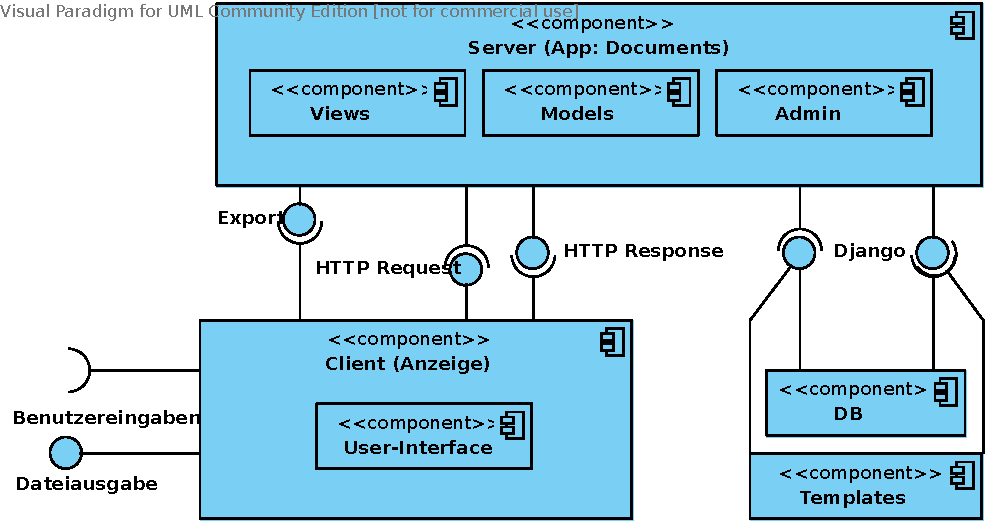
\includegraphics[width=0.8\linewidth]{bilder/Komponentendiagramm.pdf}
\caption[Komponentendiagramm]{Komponentendiagramm}
\label{Komponentendiagramm}
    \end{center}
\end{figure}

\section{Schnittstellenspezifikation}

\begin{tabular}[ht]{|l|p{0.35\linewidth}|p{0.35\linewidth}|}
\hline
Schnittstelle & \multicolumn{2}{|c|}{Aufgabenbeschreibung}\\
\hline
\hline
/S10/ HTTP Request & \multicolumn{2}{|c|}{}\\
\hline
& search(String) : List & Die Suche liefert eine Liste mit den Ergebnissen\\
& signIn(String) : boolean & Anmelden des Benutzers\\
& signOut() : boolean & Abmelden des Benutzers\\
& import(data) : boolean & Import \\
& getHistory(String) : List & liefert eine Liste der Ausgeliehen Dokumente\\
& getDoc(String) : List & liefert die Dokumentinformationen in einer Liste\\
& getView(String) : View & liefert die View, die die Aufgabenstellung erfüllt\\
\hline
/S20/Export & \multicolumn{2}{|c|}{Exportieren von Informationen}\\
\hline
& exportBibTeX() : String & Liefert einen String welcher die
Dokumentinformationen im \BibTeX -Format enthält\\
& exportAllegro() : \Gls{glos:Allegro} -kompatible Datei & Liefert eine Datei für die
\Gls{UB}\\
\hline
/S30/\gls{glos:django} & \multicolumn{2}{|c|}{Verbindung mit Datenbank}\\
\hline
& connect(String) : boolean & Verbindung zur Datenbank\\
& disconnect() : boolean & Verbindung wird beendet\\
& sendQuery(String) : List & liefert eine Liste des Ergebnisses\\
\hline
\end{tabular}





\section{Protokolle für die Benutzung der Komponenten}

In diesem Unterkapitel werden nun die Protokoll-Statecharts für alle 
Komponenten, welche in dem Komponentendiagramm \ref{Komponentendiagramm} 
vorhanden sind, dargestellt.

Für jede dieser Komponenten ist eine Wiederverwendung begrenzt sinnvoll, da alle
 diese Komponenten sehr projektspezifisch gehalten werden müssen. Sie können 
 unter Umständen in anderen Projekten eingesetzt werden, aber dann nur unter 
 größtem Anpassungsbedarf.

\subsection{Client}
\begin{figure}[H]
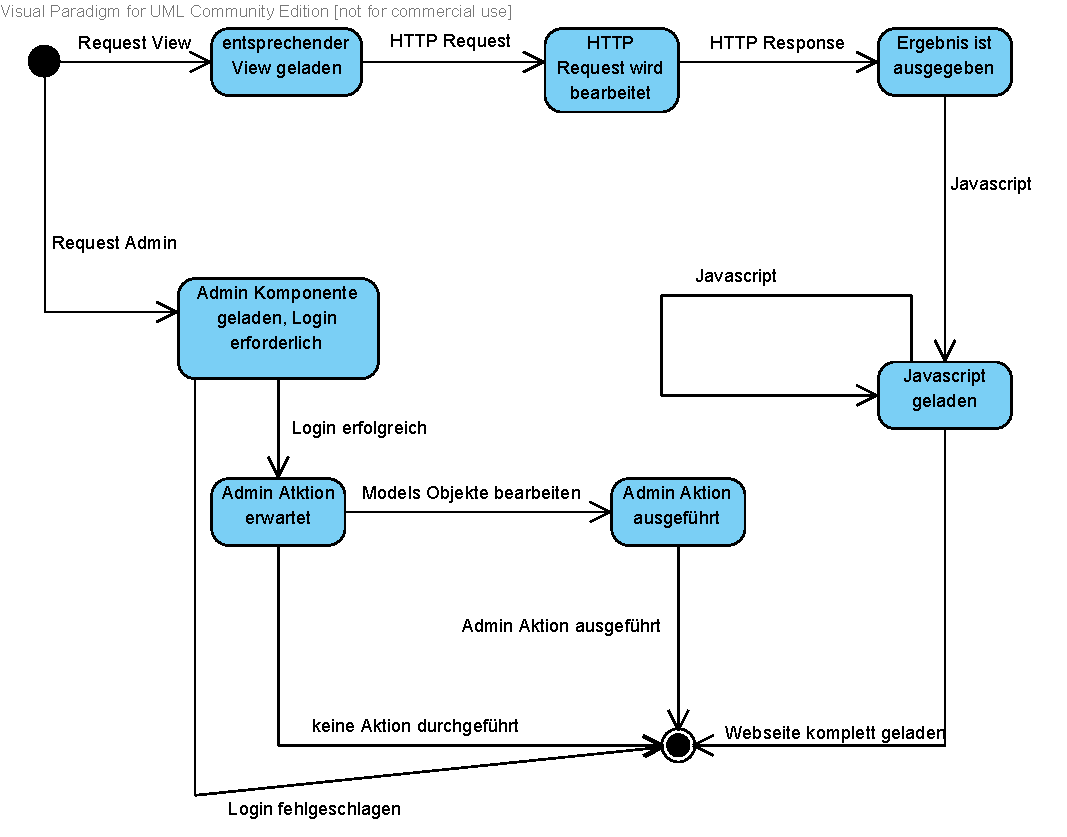
\includegraphics[width=0.8\linewidth]{bilder/KompClient.pdf}
\caption{Statechart für die Komponente Client}
\label{StClient}
\end{figure}

Vom Startzustand des Statecharts Abb.\ \ref{StClient} aus gibt es entweder die 
Möglichkeit, dass der Client eine Djangoview oder die Adminansicht aufruft. Wird 
die Adminkomponente aufgerufen, erwartet der Client zuerst eine 
Authentifizierung. Schlägt diese fehl, wird der Zugriff verweigert. Wenn sie 
aber erfolgreich ist, erwartet der Client als nächstes ein oder mehrere 
Adminaktionen oder das Beenden der Adminansicht. Ruft der Client eine Djangoview 
auf, lädt er zuerst die entsprechende View und stellt dann einen HTTP-Request. 
Sobald er das entsprechende Ergebnis erhält, gibt er es aus und lädt benötigte 
Javascripte. Damit ist die Seite komplett geladen und der Client in seinem 
Endzustand.

\subsection{View}
\begin{figure}[H]
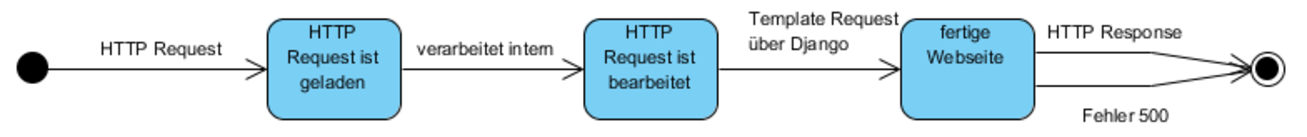
\includegraphics[width=0.8\linewidth]{bilder/KompView.pdf}
\caption{Statechart für die Komponente View}
\label{StView}
\end{figure}

Eine View (Statechart Abb.\ \ref{StView}) erhält immer zuerst einen HTTP 
Request, den sie lädt und dann verarbeitet. Ist dies geschehen, wird über das 
Djangotemplatesystem eine entsprechende fertige Webseite erzeugt und per HTTP 
Response zurückgegeben. Alternativ kann die Rückgabe auch aus einem Fehler 500 
bestehen.

\subsection{Model}
\begin{figure}[H]
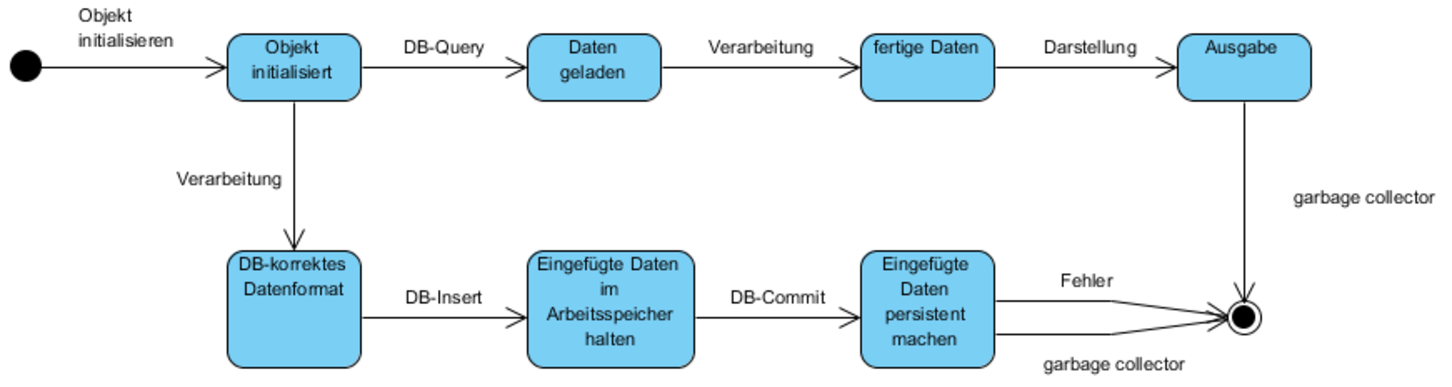
\includegraphics[width=0.8\linewidth]{bilder/KompModel.pdf}
\caption{Statechart für die Komponente Model}
\label{StModel}
\end{figure}

Nachdem das Objekt initialisiert ist, kann entweder eine Anfrage oder eine
Bearbeitung ausgeführt werden (siehe Statechart Abb.\ ref{StModel}). Wird etwas 
bearbeitet, werden die Daten zuerst in ein DB-kompatibles Format geändert. 
Nachdem DB-Insert werden die Daten noch im Arbeitsspeicher gehalten, bis der 
Commit abgeschlossen ist und die Daten konsistent gemacht wurden. Dann löscht 
der Garbage Collector das Objekt und versetzt es damit in seinen Endzustand. 
Wurde eine Anfrage gestellt, werden die Daten entsprechend der Query geladen. 
Nach der Verarbeitung der Daten und der Erstellung des Ergebnisses der Query 
wird dieses in einer Ausgabe dargestellt. Nachdem die Ausgabe beendet wurde, 
wird das Objekt vom Garbage Collector gelöscht und damit in seinen Endzustand 
versetzt.

\subsection{Admin}
\begin{figure}[H]
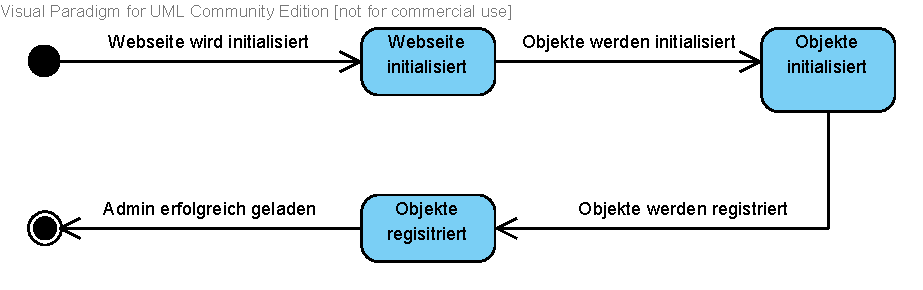
\includegraphics[width=0.8\linewidth]{bilder/KompAdmin.pdf}
\caption{Statechart für die Komponente Admin}
\label{StAdmin}
\end{figure}

Die Komponente Admin (Abb.\ \ref{StAdmin}) erstellt zuerst eine Webseite, dann 
initialisiert sie entprechende Objekte und registriert sie. Damit ist die 
Adminseite vollständig geladen. Die restliche Funktionsweise wurde bereits in 
Abb.\ \ref{StClient} beschrieben, da diese ineinander greifen.


\subsection{DB und Template}
Die Komponente \textbf{DB} wird hier nicht modelliert, da diese zunächst trivial
 ist(Anfrage an DB -> DB liefert Ergebnis) und die \textbf{DB} vollkommen durch 
 \gls{glos:django} auf die Komponente \textbf{Models} gemappt wird.

Auch auf eine Darstellung der Komponente \textbf{Template} wird verzichtet, da 
ein Template nur einen wirklichen Zustand hat, und dies ist der des Existierens. 




%In diesem Abschnitt wird mit Hilfe von Protokoll-Statecharts die korrekte
%Verwendung der zu entwickelnden Komponenten dokumentiert. Dies ist insbesondere
%für diejenigen Komponenten notwendig, für die eine Wiederverwendung möglich
%erscheint oder sogar bereits geplant ist.

%Begründen Sie für welche Komponenten eine Wiederverwendung sinnvoll erscheint
%und für welche nicht!

%Fügen Sie so viele Statechartdiagramme ein, wie sie Komponenten gefunden haben.
      % Kapitel 3
% Kapitel 4
%-------------------------------------------------------------------------------
\chapter{Verteilungsentwurf}
Da es sich bei dem Produkt um eine Datenbank-basierte Webanwendung handelt, liegt hier ein verteiltes System in Form eines Client-Server-Modells vor:

Durch eine Ressource-Anforderung (request) mithilfe eines Webbrowsers benutzt der Client über eine IP (oder einem Servernamen) die Adresse des Servers. Dieser gibt den Request an den Webserver weiter.
Mithilfe des Servers beanwortet der Webserver schließlich den Request und schickt das Ergebnis (response) an den Client zurück.   

        % Kapitel 4

%---Hier werden das Glossar und das Abkürzungsverzeichnis gedruckt--------------
\providetranslation{Glossary}{Glossar}
\printglossary[style=altlist,title=Glossar]

\providetranslation{Acronyms}{Akronyme}
\printglossary[type=\acronymtype,style=long]


%------Ende des Dokumentes------------------------------------------------------
\end{document}
